% Working chapter, 2026-10-24. Source checked against arXiv:2406.00318v1.
% The author confirmed that the linked arXiv PDF is publication-equivalent.
% Status AUTHOR_CONFIRMED_PUBLICATION_EQUIVALENT; not a direct publisher download.
% Author instruction: use publication prose to resolve internal prose/table conflicts.
% Detailed verification, source omissions, and remaining QA are in planning/verification-kglink.md.
\chapter{Knowledge-enriched Table Understanding with KGLink}
\label{ch:kglink}

This chapter is based on the published paper \emph{KGLink: A Column Type Annotation Method that Combines Knowledge Graph and Pre-Trained Language Model}~\cite{kglink-publication}. It studies how a knowledge graph can supply information missing from a table and how a pre-trained language model can translate that information into the type vocabulary of a particular annotation task. The prediction target is a column label. Graph evidence enters the model through candidate types and a separate feature sequence, while a supervised representation task connects the evidence to the dataset's annotation scheme.

\section{Motivation and Task}
\label{sec:kglink:motivation}

A table often presents entities through short names, abbreviated strings, or numbers. These values provide only part of the information needed to identify a column's semantic type. A column containing names of cricket players may appear beside birth and death dates. Those dates describe the people but do not specify their occupation. A language model that encodes only the table receives a different evidential basis from a model that also has access to relations such as occupation and sport in a knowledge graph. The annotation problem therefore concerns both interpreting the available text and selecting external information that clarifies it.

External knowledge introduces a second difficulty. The type expected by an annotation dataset need not coincide with a type attached to an entity in the graph. A column of basketball players can plausibly be described as \emph{Basketball player}, \emph{Athlete}, or \emph{Name}. An annotation benchmark may use only the last of these labels. Retrieving a factually relevant graph type is consequently insufficient to determine the required output label. The model must learn which description the task expects. KGLink refers to this mismatch as the type granularity gap. The gap includes cases where the desired dataset label does not occupy a convenient ancestor position in the retrieved graph's type hierarchy.

These two difficulties give structure distinct roles. Relations between linked entities can help identify relevant knowledge, while supervised learning can determine how that knowledge should influence a dataset-specific prediction. Treating graph types as final labels combines those roles too early. Treating the table as an isolated sequence omits the external relations. KGLink keeps graph evidence available to a learned classifier and trains an auxiliary task that generates a contextual representation of the target type. The learned classifier maps graph-derived evidence into the task's output classes.

The scope of the chapter is column-type annotation on the evaluated SemTab and modified VizNet datasets. Reasoning takes the form of inferring a semantic category from cells, their table context, and graph-derived evidence. The language model is an encoder trained for classification. Its output is drawn from the dataset's label set. This task establishes the first setting examined in the thesis, where an existing graph augments a model's representation before prediction.

\begin{figure}[tbp]
\centering
\begin{minipage}[b]{0.48\linewidth}
\centering
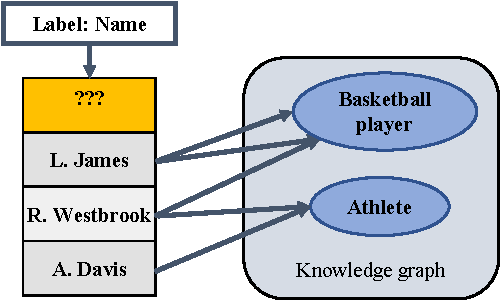
\includegraphics[width=\linewidth]{figures/kglink/tg_issue_small.pdf}
\par\small (a) Type granularity
\end{minipage}\hfill
\begin{minipage}[b]{0.48\linewidth}
\centering
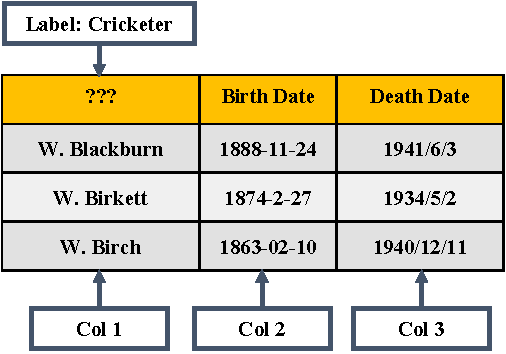
\includegraphics[width=\linewidth]{figures/kglink/DL_NotWell_small.pdf}
\par\small (b) Missing context
\end{minipage}
\caption{Two annotation difficulties in the original KGLink examples. A graph description such as Athlete can differ from the target label Name, while dates beside a person's name provide little occupation information. Original subfigures reproduced from KGLink~\cite{kglink-publication}, Fig.~2.}
\label{fig:kglink:motivation}
\end{figure}

\section{Problem Formulation and Framework}
\label{sec:kglink:problem}

Let $T$ be a table with row set $R$ and column set $C$. A cell mention $m_c^r$ is the content of row $r$ and column $c$. The task assigns a label $l_c$ from the dataset's type set $D$ to each target column. All columns in the same table can contribute context to that decision. The external knowledge graph supplies entity labels and their one-hop relations. During training, column labels supervise both classification and the auxiliary representation task. During evaluation, those labels are absent from the model input.

KGLink has a graph-processing stage followed by a language-model stage. The graph stage retrieves candidate entities for cell mentions, filters these entities using connections between columns, ranks rows by their linkage quality, and derives candidate types from the remaining entities' neighborhoods. It also constructs a feature sequence for each target column. The language-model stage serializes the processed table, encodes the table and feature sequences, combines the resulting representations, and predicts the column labels. A second training input contains the true type labels and provides contextual supervision for representations generated from masked type positions.

Figure~\ref{fig:kglink:framework} shows the two stages and their training objectives.

\begin{figure}[tbp]
\centering
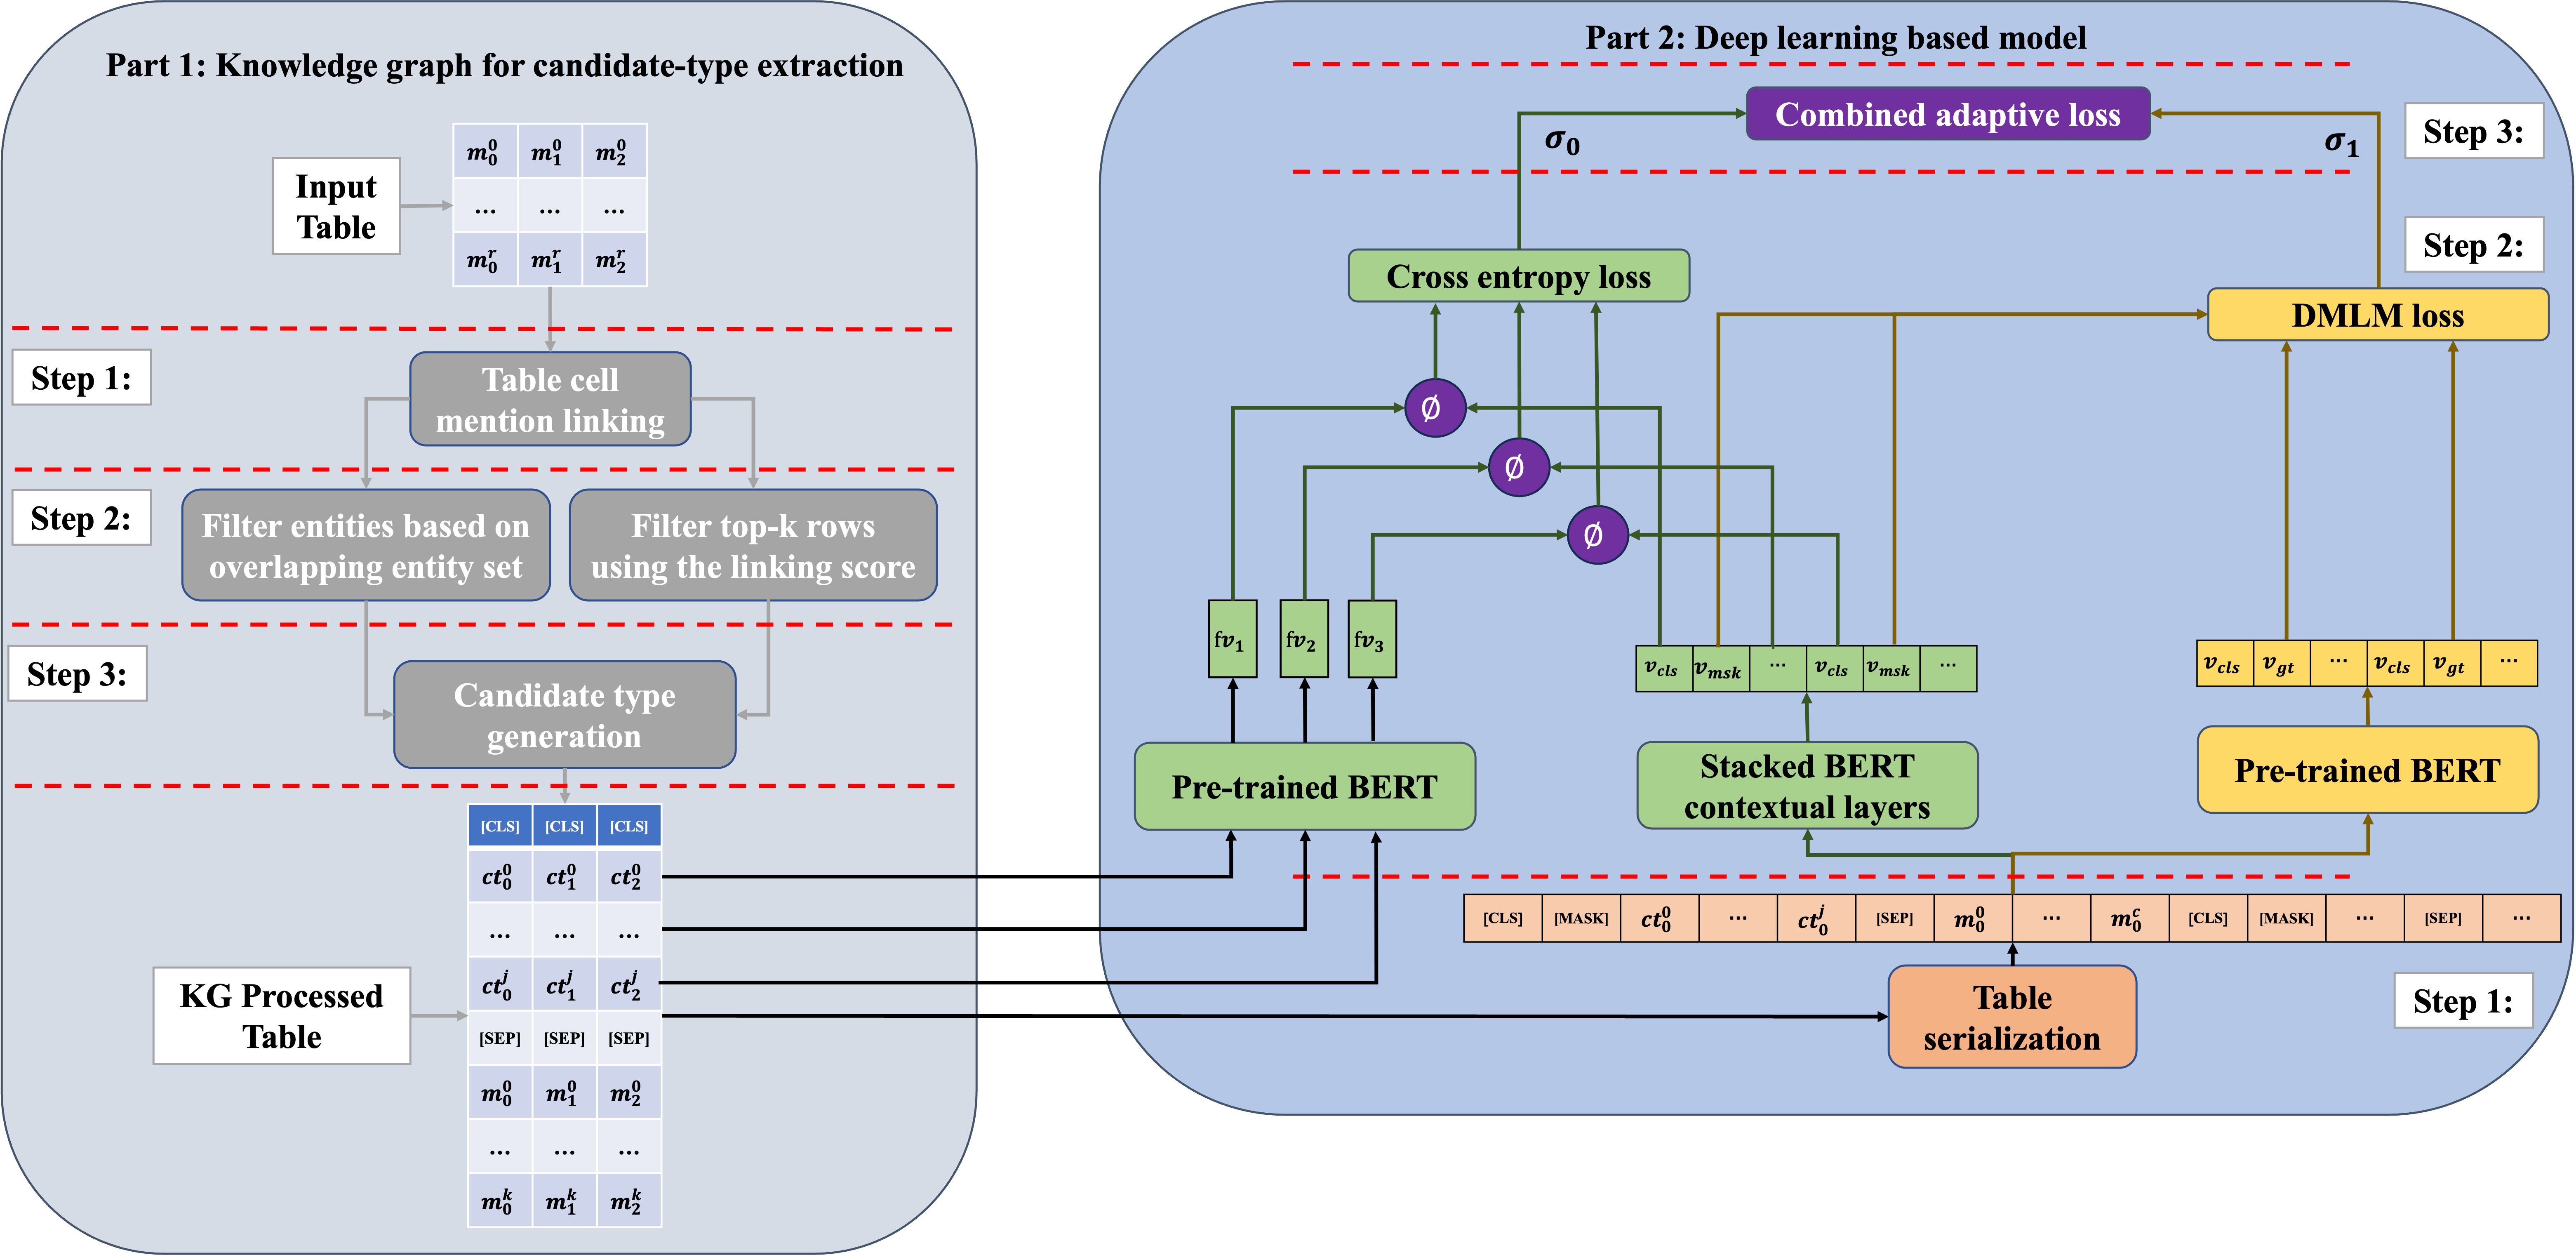
\includegraphics[width=\linewidth]{figures/kglink/kglink_new_overview.png}
\caption{KGLink's graph-processing and language-model components. Candidate-type text, column feature vectors, and a contextual type-representation objective connect external knowledge to annotation. Original image reproduced from KGLink~\cite{kglink-publication}, Fig.~3.}
\label{fig:kglink:framework}
\end{figure}

The two graph inputs have different selection rules. Candidate types aggregate evidence across linked cells and retain types supported by the column. A feature sequence describes a selected linked entity and its neighboring relations. The latter supplies another route for KG information when candidate-type selection produces little evidence. Neither input changes the classifier's output vocabulary. For example, a candidate type describing an occupation can support a broader annotation category through the learned model even when the strings differ.

The framework also controls the amount of table content passed to the encoder. Entity linking and row selection precede serialization. The retained rows provide a bounded view of the table, and wide tables are split by columns under the reported input constraints. These operations matter because inserting external knowledge competes with cell content for the encoder's finite input length. KGLink selects graph evidence and table rows before encoding.

\section{KG-derived Candidate Types}
\label{sec:kglink:candidates}

\subsection{Cell Mention Linking}
\label{sec:kglink:linking}

The first step retrieves a candidate entity set $E_{m_c^r}$ for each suitable cell mention. KGLink uses BM25 to score the relation between the mention's words and indexed entity labels~\cite{kglink-robertson2009probabilistic}. The implementation indexes Wikidata with Elasticsearch. The score incorporates query-term frequency, inverse document frequency, and label-length normalization. Multiple entities can match the same mention, so the retrieval output is a candidate set rather than a single disambiguated entity.

This distinction is relevant for short strings. An album title and an ordinary word may share the same surface form, while a person's name can refer to several people. Lexical matching can identify plausible entries without determining which one belongs in the current table. KGLink uses the table's row structure in the next step to provide this disambiguating context. A cell's candidate set is consequently an intermediate object whose members can be removed when their graph relations disagree with evidence from other columns.

Numeric and date mentions are handled separately. The reported procedure uses named-entity detection to identify these mentions and assigns them a linking score of zero. A failed entity lookup also receives a zero linking score. The subsequent model still receives the table values, so absence of a graph link does not remove a column from the annotation task. The language-model component provides the classification pathway for columns with missing KG evidence.

The experimental implementation retrieves at most ten entities per cell mention. This limit bounds the candidate sets that enter the subsequent neighborhood operations. Graph-based filtering and row ranking select among the retrieved evidence before it reaches the annotation model.

\subsection{Cross-column Neighborhood Filtering}
\label{sec:kglink:filtering}

\begin{figure}[tbp]
\centering
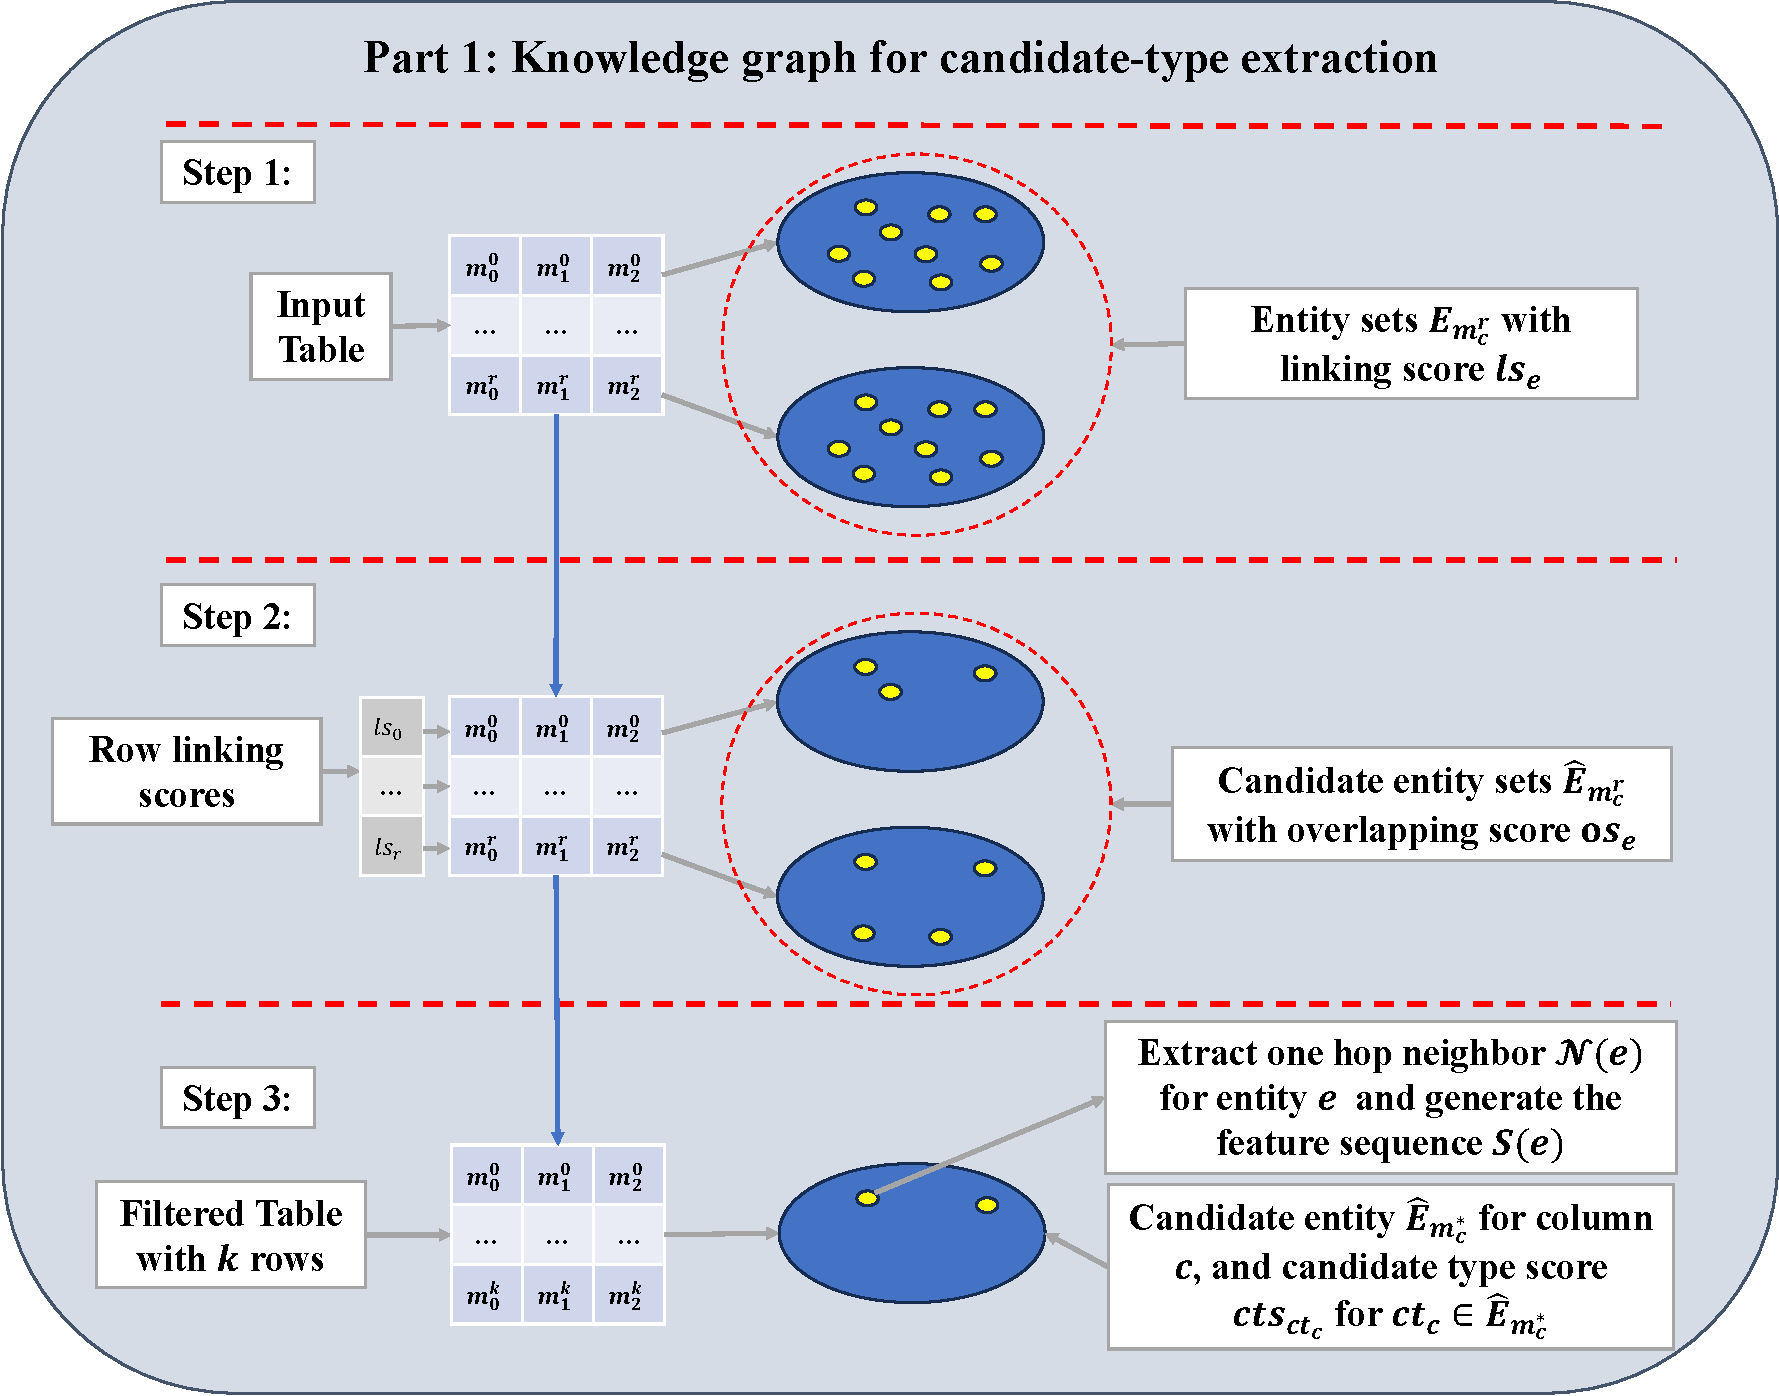
\includegraphics[width=0.76\linewidth]{figures/kglink/KG_part.pdf}
\caption{The original KG-processing pipeline. Cell linking is followed by entity filtering, row selection, and candidate-type generation. Reproduced from KGLink~\cite{kglink-publication}, Fig.~4.}
\label{fig:kglink:kg-pipeline}
\end{figure}

Cells in the same row describe related objects. An album title beside a musician's name supplies a useful relation that either mention lacks in isolation. KGLink uses this relation by checking whether a candidate entity for one cell occurs in the one-hop neighborhood of candidates for another cell in the same row. Let $\mathcal{N}(E)$ denote the one-hop neighbors of a candidate entity set. The filtered set for a cell is
\begin{equation}
\widehat{E}_{m_{c_1}^{r}}
 = \bigcup_{c_2\in C\setminus\{c_1\}}
 \left(E_{m_{c_1}^{r}}\cap\mathcal{N}(E_{m_{c_2}^{r}})\right).
\label{eq:kglink:entity-filter}
\end{equation}
The union allows support from any other column. The intersection retains entities retrieved for the target mention that also have the required neighborhood support.

Figure~\ref{fig:kglink:overlap} uses \emph{Rust} and \emph{Peter Steele}. A graph connection between an album candidate and the musician candidate supports their interpretation as the entities intended by the row. The role of the edge is to constrain which external facts are relevant to the table. KGLink subsequently associates each retained entity with an overlapping score that counts its neighborhood support from other columns. Entities with more such support contribute more to candidate-type selection.

Neighborhood support is a structural selection signal. It depends on the relations recorded in the external graph and on the initial entity candidates. A missing graph relation can remove useful evidence, while an incorrect lexical candidate can survive if it has matching contextual links. The model therefore also uses the original table sequence and a separate feature representation. This architecture gives graph filtering a specific responsibility, selecting evidence for the classifier, without making its output the classifier's final decision.

\begin{figure}[tbp]
\centering
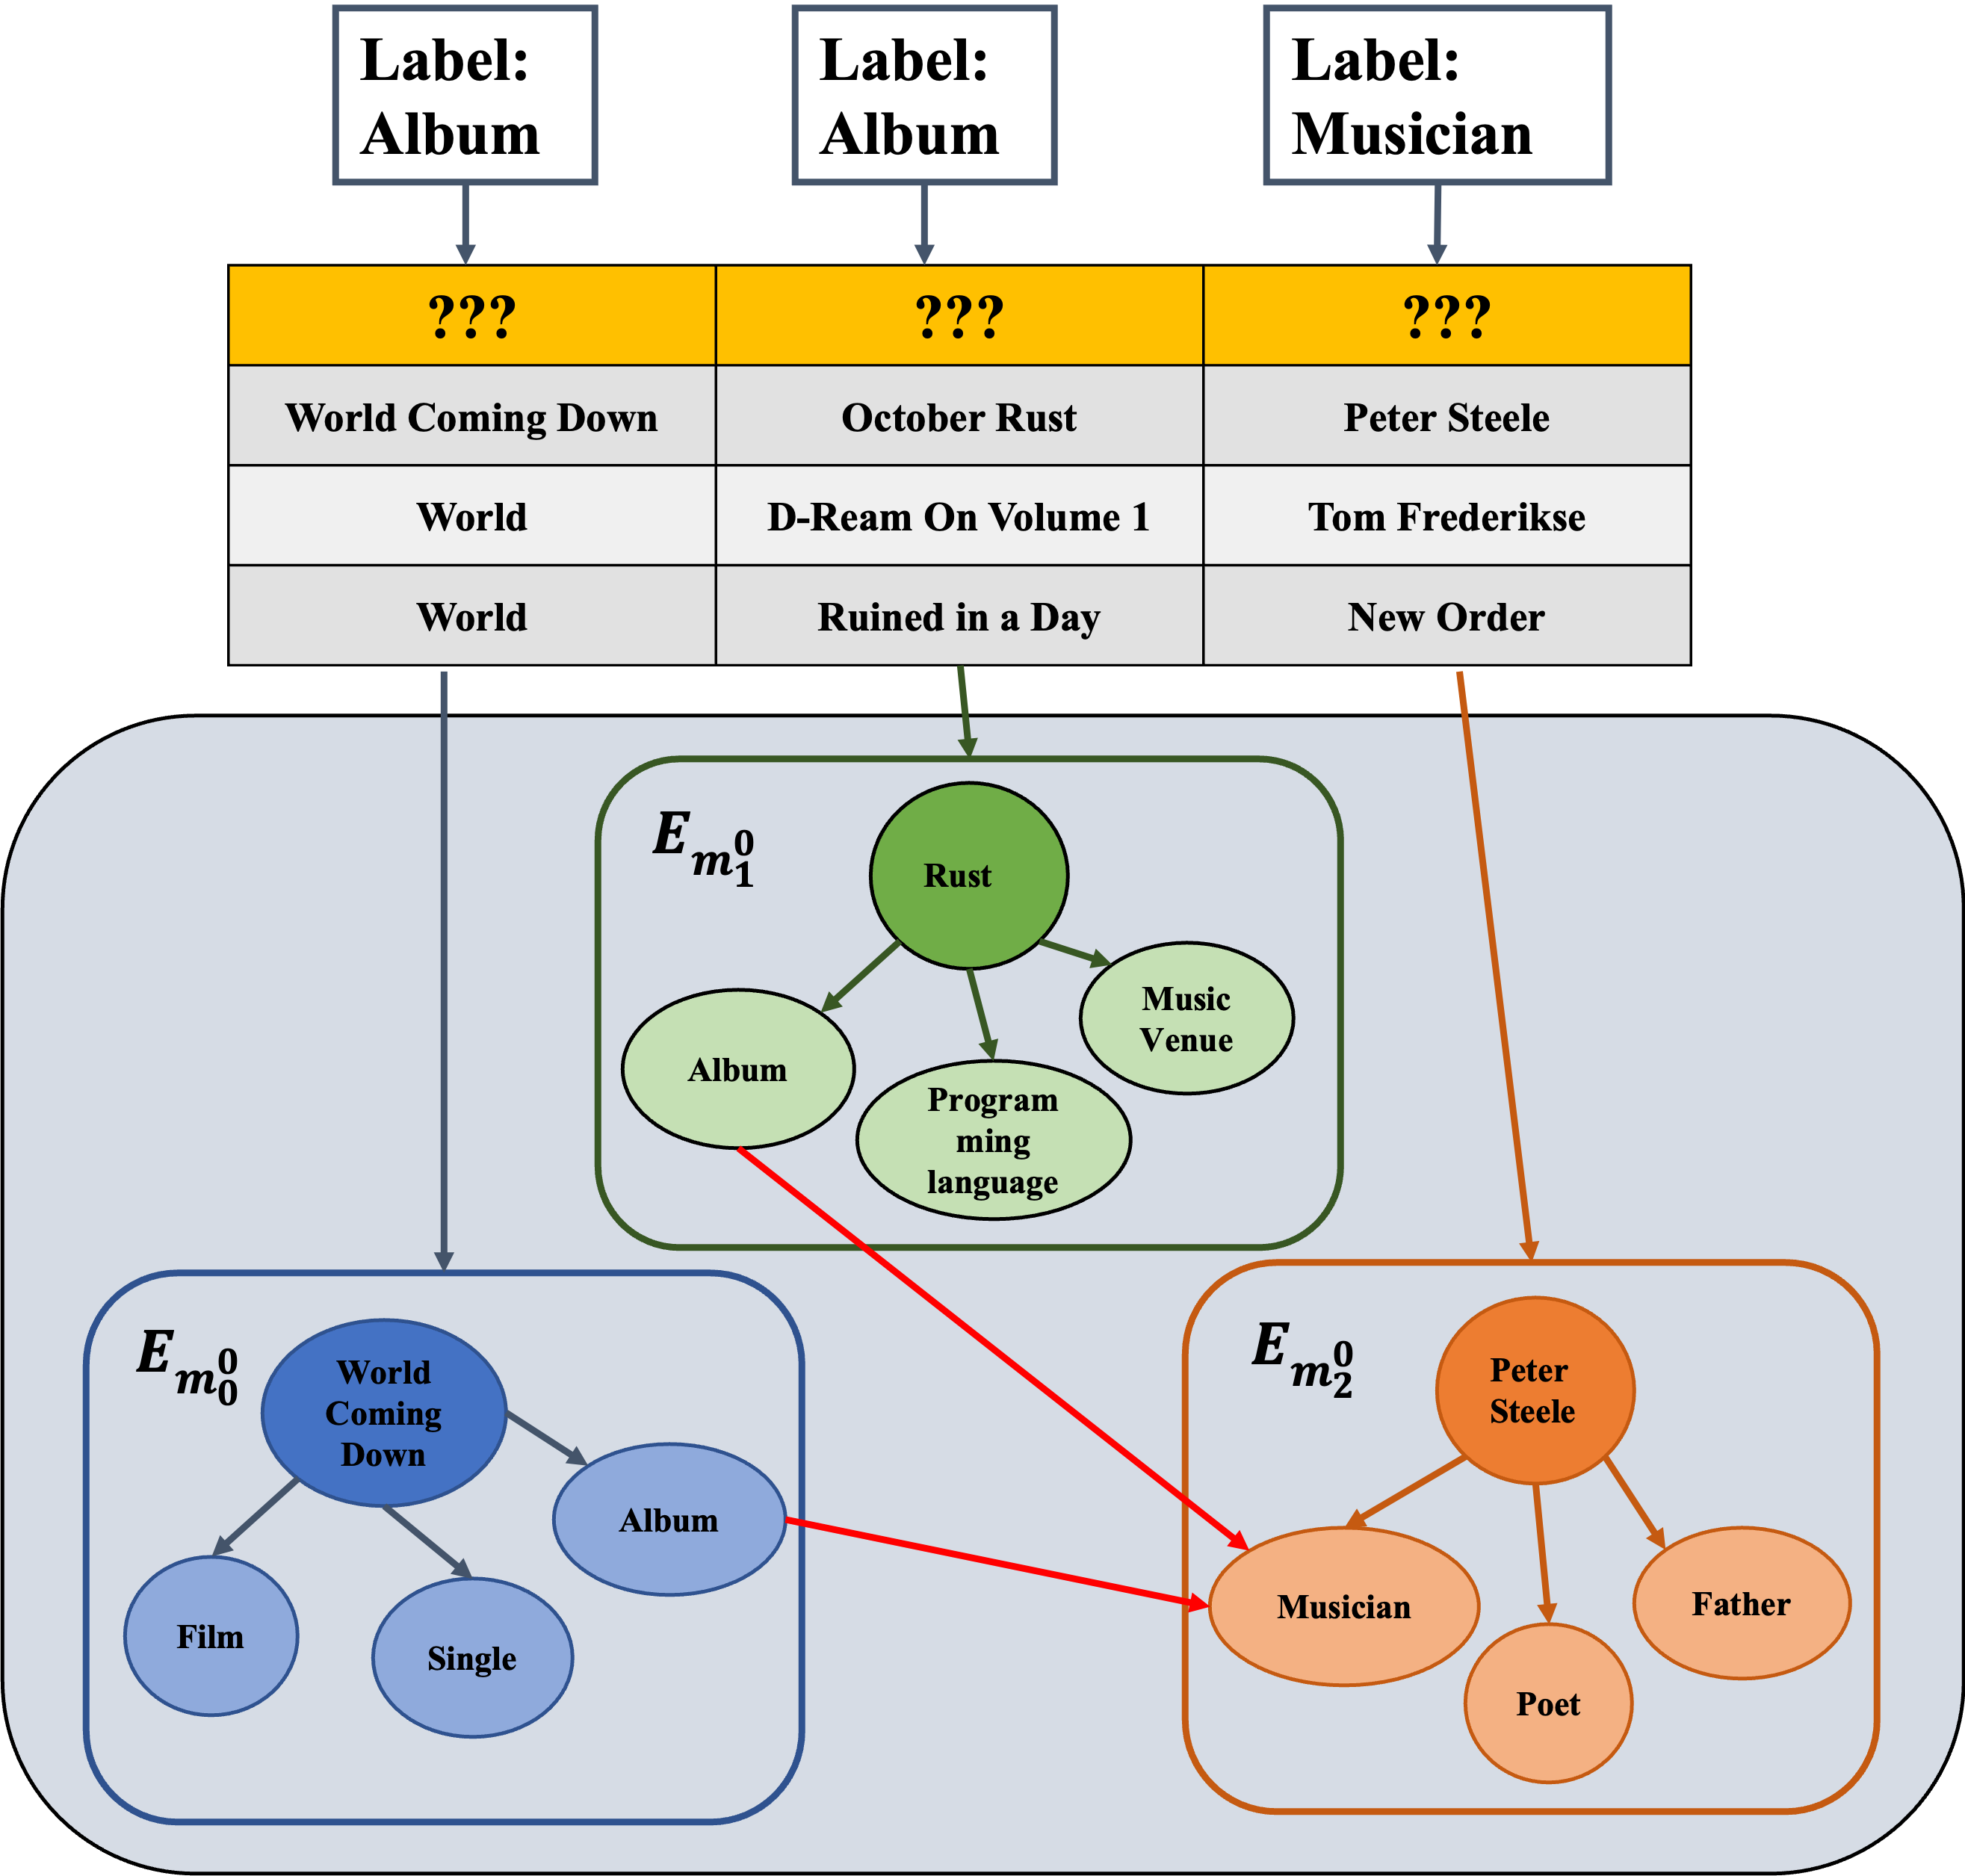
\includegraphics[width=0.75\linewidth]{figures/kglink/overlap.png}
\caption{Cross-column evidence in the original album-and-musician example. Graph links connect candidate interpretations of cell mentions in the same row. Original image reproduced from KGLink~\cite{kglink-publication}, Fig.~5.}
\label{fig:kglink:overlap}
\end{figure}

The filter uses inter-column information within a row, whereas candidate-type generation aggregates across rows within a column. These are different structural assumptions. The first exploits the relation between attributes of the same record. The second looks for recurring semantic descriptions of several values occupying the same column. Separating them clarifies why a relevant neighbor of one entity is insufficient on its own to determine a column's type.

\subsection{Row Linking Quality and Input Selection}
\label{sec:kglink:rows}

KGLink derives a cell score from the best-scoring retained entity. For a nonempty filtered candidate set, the score is
\begin{equation}
ls_{m_c^r}=\max_{e\in\widehat{E}_{m_c^r}}ls_e,
\label{eq:kglink:cell-score}
\end{equation}
where $ls_e$ is the entity's BM25 linking score. Unlinked cells use zero as described in the evaluation protocol. A row's score sums the scores of its cells,
\begin{equation}
ls_r=\sum_{c\in C}ls_{m_c^r}.
\label{eq:kglink:row-score}
\end{equation}
Rows are sorted by this quantity, and only the top $k$ rows are retained for prediction.

This operation changes which examples of a column the language model observes. Selecting the first $k$ rows preserves the source table's order; ranking by linkage favors rows with more lexically supported graph evidence after filtering. The latter can make the external evidence more useful within the same row budget. The row-filter experiment compares the two selection rules while retaining the reported input limit.

Row selection also connects the graph and feature pathways. The feature sequence is generated from a selected cell associated with the highest-ranked row. Changing the row order can therefore affect the table content and the KG entity used to form that sequence. The row-selection experiment evaluates this coupled selection mechanism.

\subsection{Candidate Types and Feature Sequences}
\label{sec:kglink:types-features}

Candidate-type generation searches beyond an entity's explicit type attribute. A person's graph entry may be typed as \emph{Human}, while \emph{Musician} appears as an occupation neighbor. The latter can be more informative for a table column. KGLink collects filtered entities across the target column and examines their one-hop neighborhoods. It scores a potential type by aggregating the overlapping scores of entities from other rows that connect to that type. Repeated support within the column increases the candidate's score.

A label-based filter excludes candidates assigned the named-entity schema categories \texttt{PERSON} or \texttt{DATE}. The reported implementation uses spaCy for this step. This filter distinguishes a descriptive candidate type from a particular person's name or a date encountered in the neighborhood. KGLink retains the selected candidate-type labels as text and places them before the cell values in the processed column. The reported implementation generates up to three candidate types per row from the KG entities in each column. Their later contribution depends on how the encoder interprets them in the table context.

If no candidate type is returned, padding occupies the corresponding position. Numeric columns use numeric summary information in this part of the input, while their original values remain available in the table sequence.
% Source issue: “mean, variance, and average value” duplicates mean/average.
% Keep the exact list out of final method specification until author/publisher resolution.

The feature sequence provides a second representation of the retrieved knowledge. From the filtered and ranked table, KGLink selects a cell for each target column, chooses its highest-linking entity, and serializes that entity with its one-hop predicates and neighboring entities. If $e$ is the selected entity, $p$ a predicate, and $o$ a neighboring object, the sequence consists of the entity label followed by predicate--object descriptions. Encoding this text yields a feature vector for the column. A padding sequence is used when the column has no retrieved entity.

Candidate types and feature sequences thus preserve different aspects of a neighborhood. Candidate selection emphasizes descriptions recurring across column values. The feature sequence retains relational details surrounding a particular well-linked value. The experimental ablations examine the two pathways through specific model variants.

\section{Language Model Integration}
\label{sec:kglink:language-model}

\subsection{Table Serialization and Column Representations}
\label{sec:kglink:serialization}

KGLink adapts the multi-column serialization used by Doduo~\cite{kglink-suhara2022annotating}. A special \texttt{[CLS]} token begins each column's segment. The segments are concatenated into one input sequence, followed by a \texttt{[SEP]} token. The contextual representation at each column's \texttt{[CLS]} position provides that column's vector. Because the sequence contains multiple columns, self-attention can use information outside the predicted column.

Writing the tokenized contents of column $i$ as $\mathrm{tok}_i^1,\ldots,\mathrm{tok}_i^{m}$, the original multi-column serialization has the form
\begin{equation}
\begin{split}
S(T)={}&[\mathrm{CLS}]\ \mathrm{tok}_1^1\cdots\mathrm{tok}_1^m\ 
[\mathrm{CLS}]\ \mathrm{tok}_2^1\cdots\\
&[\mathrm{CLS}]\ \mathrm{tok}_{|C|}^1\cdots\mathrm{tok}_{|C|}^m\ 
[\mathrm{SEP}].
\end{split}
\label{eq:kglink:serialization}
\end{equation}
Each column's \texttt{[CLS]} position produces a contextual vector using the serialized columns. Candidate-type text precedes the corresponding cell values, allowing both to interact with neighboring columns through self-attention. KGLink separately encodes the feature sequence into a column-specific vector and combines it with the contextual column vector through the composition function $\phi$. The resulting representation is mapped into the dataset's classification space.

The principal experiments fine-tune BERT~\cite{kglink-devlin2018bert}. The model has a sequence limit of 512 tokens; the reported implementation limits each column to 64 tokens and each encoded table to eight columns. Tables with more columns are divided after candidate-type generation and are encoded separately. These limits define the context available to the classifier. In particular, retaining 25 table rows does not imply that every token in those rows survives serialization, since tokenization and the column limit also constrain the final sequence.

\subsection{Contextual Type Representation Learning}
\label{sec:kglink:representation}

The auxiliary task trains a type representation at a masked position. During training, KGLink constructs two versions of the processed table. The ground-truth version places the annotated type label before the candidate types in each target column. The masked version replaces that label with \texttt{[MASK]}. Both versions retain the column values and candidate-type context. Encoding the two sequences produces contextual representations for the true type and its masked counterpart.

Figure~\ref{fig:kglink:representation} illustrates the two inputs and their contextual outputs.

\begin{figure}[tbp]
\centering
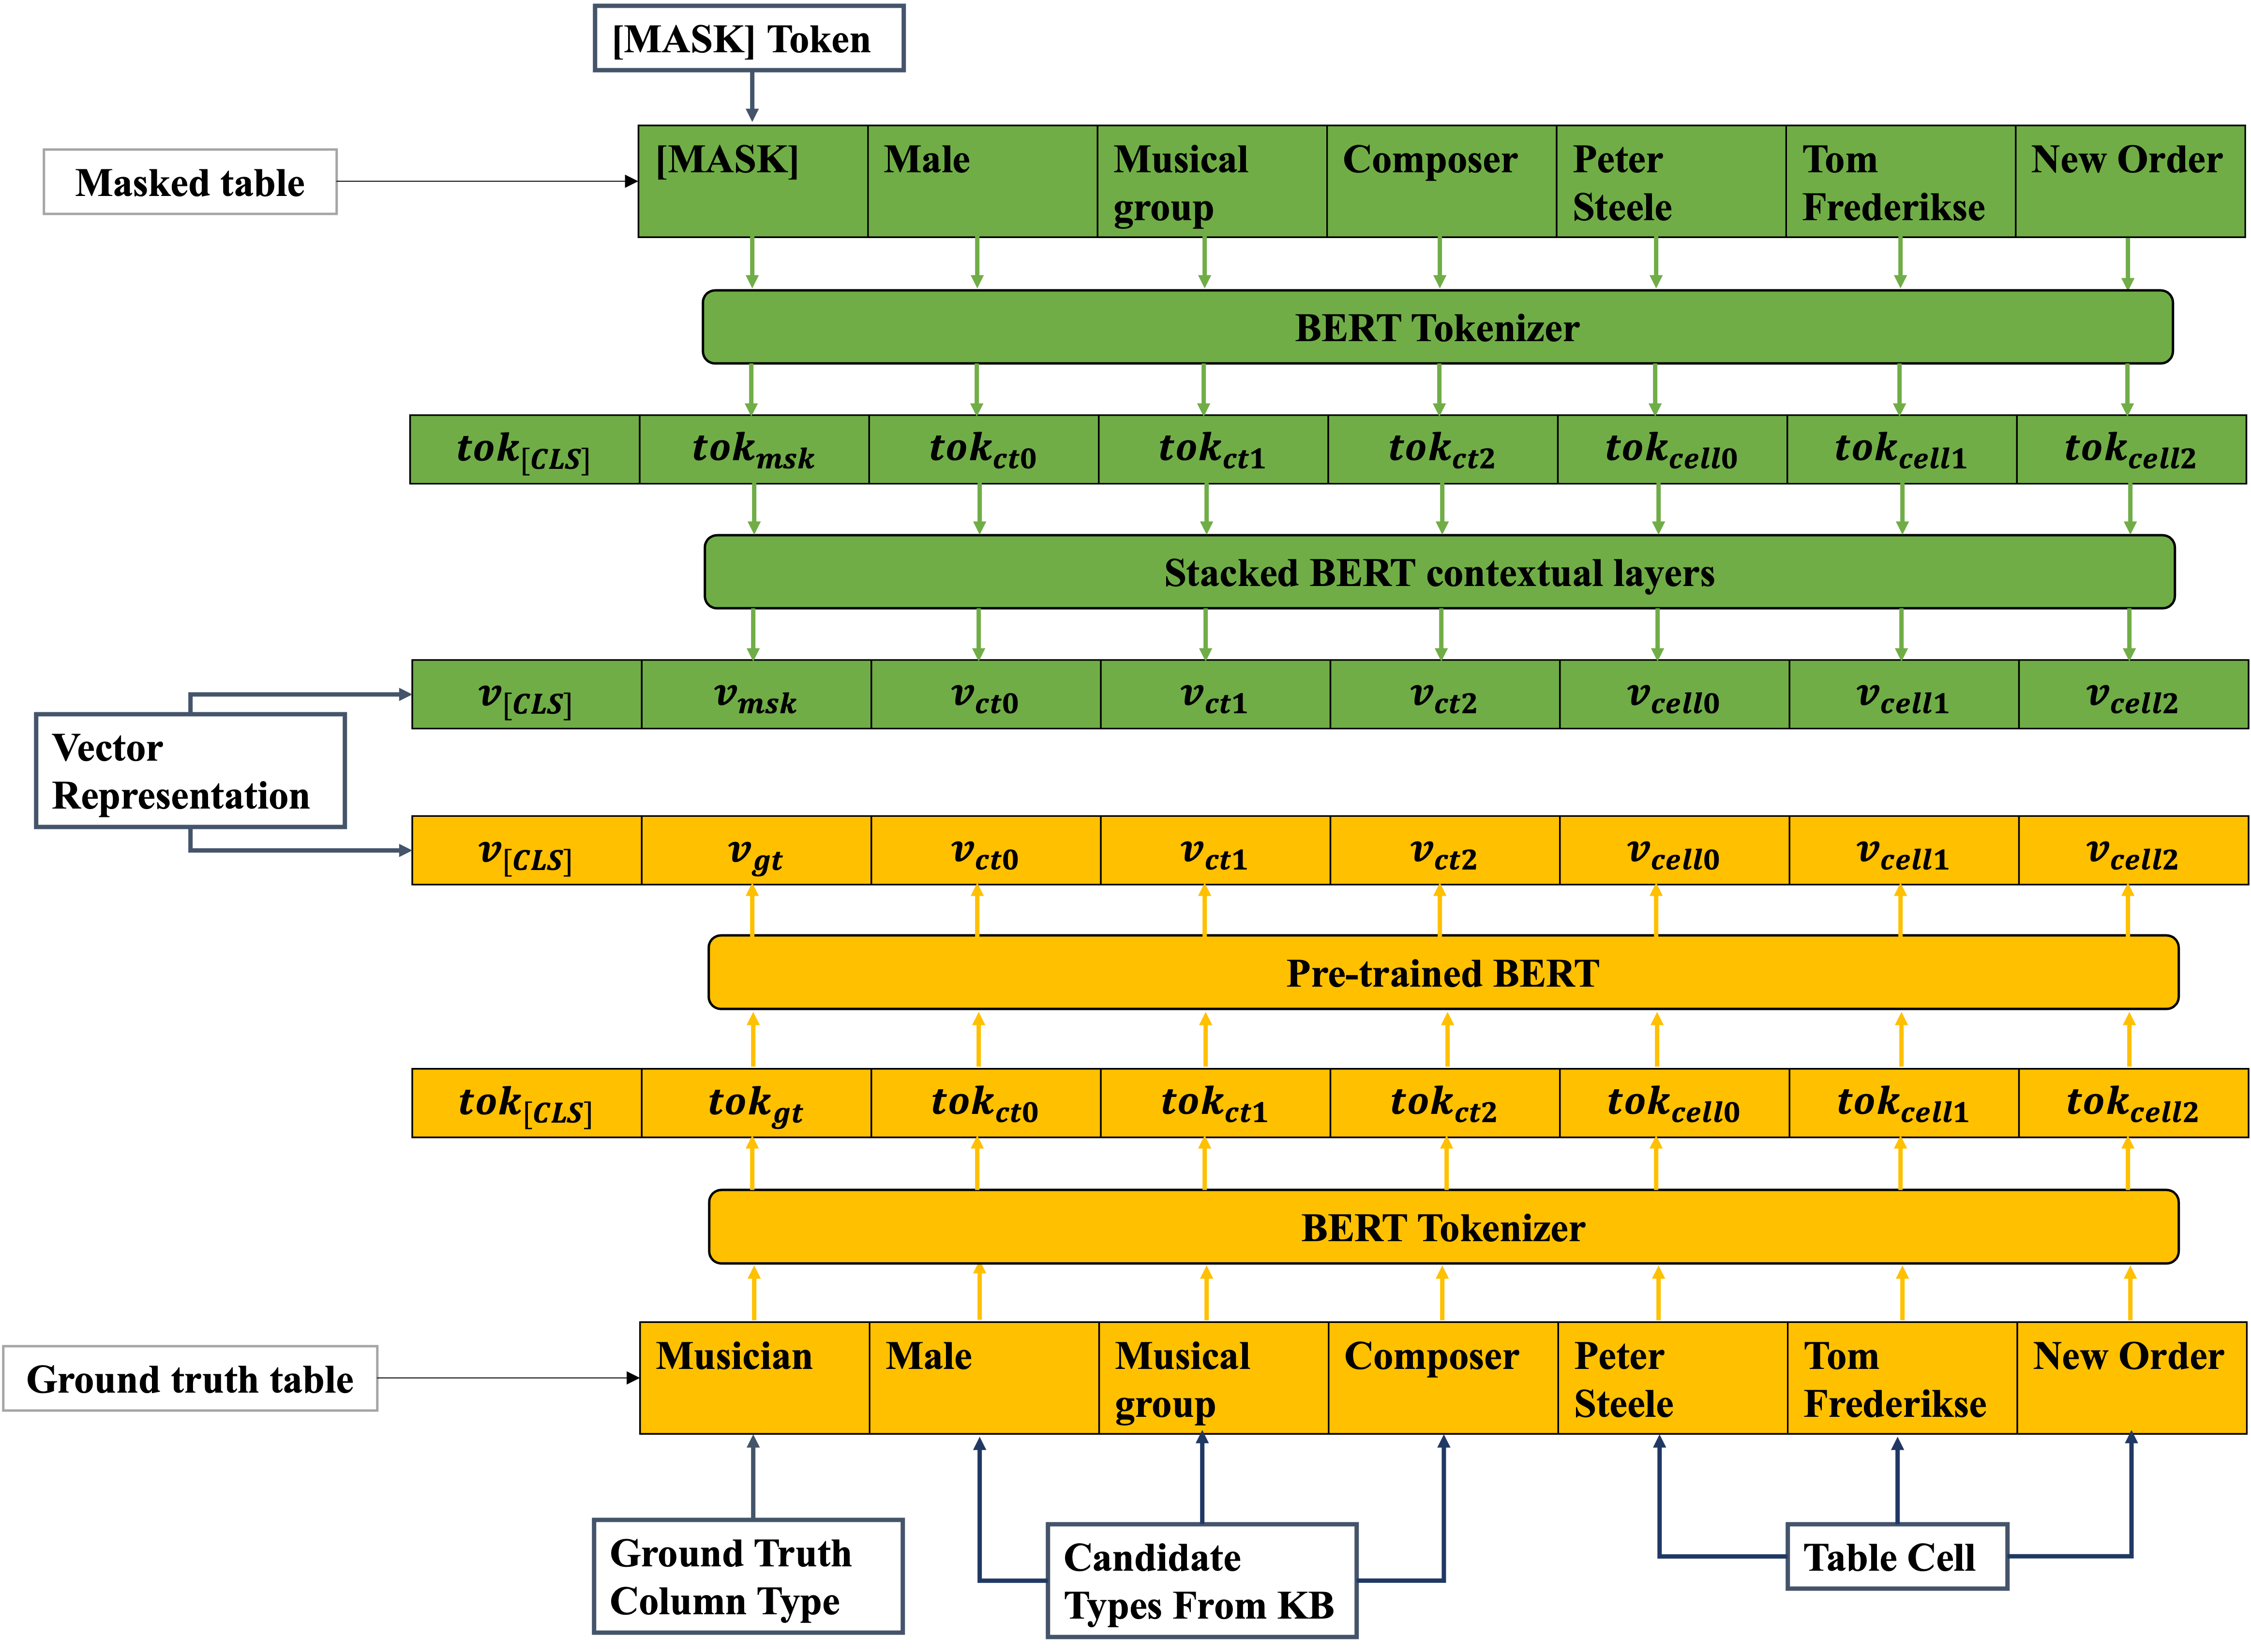
\includegraphics[width=\linewidth]{figures/kglink/dmlm.png}
\caption{Contextual type-representation training with masked and ground-truth table inputs. The true-type table is constructed during training. Original image reproduced from KGLink~\cite{kglink-publication}, Fig.~6.}
\label{fig:kglink:representation}
\end{figure}

This arrangement supplies supervision about the label's meaning in context. A label such as \emph{Musician} is encoded together with the column values and graph-derived descriptions, rather than as an isolated word. The masked input must produce its type representation from the evidence that will be available at prediction time. Distilled masked language modeling provides the auxiliary objective~\cite{kglink-wang2020learning}. The model projects contextual representations into vocabulary space with a temperature parameter, then uses the ground-truth and masked outputs in the reported training loss.

With contextual vector $H$ and temperature $\mathcal{T}$, vocabulary projection gives
\begin{equation}
Y=\operatorname{Softmax}\!\left(W_o\frac{H}{\mathcal{T}}\right),
\label{eq:kglink:vocabulary-projection}
\end{equation}
where $W_o$ projects into the vocabulary space. Denote the masked and ground-truth outputs by $Y_{\mathrm{msk}}$ and $Y_{\mathrm{gt}}$. The main paper writes the auxiliary objective as
\begin{equation}
\mathcal{L}_{\mathrm{DMLM}}(Y_{\mathrm{msk}},Y_{\mathrm{gt}})
=-\sum_{j=1}^{V}y_{\mathrm{msk}}^{j}\log y_{\mathrm{gt}}^{j},
\label{eq:kglink:dmlm}
\end{equation}
with vocabulary size $V$. The objective uses the contextualized representations produced from the two table inputs.

Training uses the true-type and masked inputs, while evaluation uses the masked input. The auxiliary objective therefore learns from labels available in training and generates a type representation from the ordinary table and retrieved evidence at prediction time. This pathway also serves numeric columns and columns without a retrieved KG candidate.

The classifier and the auxiliary task also use different output spaces. Classification predicts one of the dataset's column labels. The auxiliary representation is projected into the language model's vocabulary space. Their relationship is learned through the shared encoder and joint training. The final decision uses the dataset-specific classification head.
% Author directed main-text precedence; Eq. dmlm preserves source order exactly.

\subsection{Classification and Adaptive Task Weighting}
\label{sec:kglink:objective}

Let $z_c$ be the classification logits obtained from the combined column and feature representations. For a target label $l_c$, the classification loss is cross-entropy,
\begin{equation}
\mathcal{L}_{\mathrm{CE}}(z_c,l_c)
 =-\log\frac{\exp(z_{c,l_c})}{\sum_{j\in D}\exp(z_{c,j})}.
\label{eq:kglink:classification}
\end{equation}
KGLink jointly optimizes this loss and the auxiliary representation objective using uncertainty weighting~\cite{kglink-kendall2018multi}. With trainable task parameters $\sigma_0$ and $\sigma_1$, the combined objective is
\begin{equation}
\mathcal{L}_{\mathrm{total}}
 =\frac{\mathcal{L}_{\mathrm{DMLM}}}{2\sigma_0^2}
  +\frac{\mathcal{L}_{\mathrm{CE}}}{2\sigma_1^2}
  +\log(\sigma_0\sigma_1).
\label{eq:kglink:joint-loss}
\end{equation}
The temperature used in the representation objective is set to two in the reported experiments.

The trainable weights allow the two objectives to contribute at different scales during optimization. They weight the training objectives, while row linking scores govern input selection. These mechanisms connect graph evidence to prediction at different stages of the pipeline.

\section{Computational Structure}
\label{sec:kglink:complexity}

The graph-processing cost depends on table dimensions, candidate-set sizes, and neighborhood sizes. Linking traverses table cells. Cross-column filtering compares candidate information between columns within a row. Candidate-type scoring visits neighborhoods and aggregates support across rows. The implementation's limits on retrieved entities and serialized columns constrain these operations in the evaluated setting. The external Wikidata index is prepared with Elasticsearch and supplies lexical retrieval scores.

The original analysis denotes maximum table rows and columns by $R$ and $C$, the number of tables by $T$, the maximum retrieved entities by $E$, and their maximum one-hop neighborhood size by $N$. It reports the preprocessing expression
\begin{equation}
O\!\left(RCE(N+CET)\right).
\label{eq:kglink:preprocessing}
\end{equation}
The expression includes neighborhood aggregation and the cross-column candidate operations. It makes explicit that table dimensions and graph retrieval size affect preprocessing even when the later encoder length is capped. An increased candidate-set limit changes the graph-processing workload before any table tokens are encoded.

Encoding cost depends on the serialized input length and the encoder's hidden dimension. KGLink encodes table inputs and column feature sequences; training also includes the ground-truth and masked constructions used by the representation task. The classification head maps column vectors into the label space, while the auxiliary projection operates over the language model's vocabulary. Thus, increasing the label set affects classification, whereas increasing the vocabulary-space projection concerns the representation objective.

These costs describe different resources. Reducing the retained row count can shorten preprocessing or input preparation without proportionally changing a sequence already truncated to its token limit. Increasing candidate retrieval can add neighborhood work even when the encoder input remains fixed. The runtime and row-budget studies should therefore be read alongside the input protocol. The measurements use the reported input bounds and hardware.

\section{Experimental Evaluation}
\label{sec:kglink:experiments}

\subsection{Datasets and Protocol}
\label{sec:kglink:protocol}

The evaluation uses SemTab 2019 and a modified VizNet subset~\cite{kglink-hassanzadeh_oktie_2019_3518539,kglink-zhang2020sato}. SemTab includes tables derived from Wikipedia, DBpedia, and the T2Dv2 Gold Standard sources. The experiment uses rounds 1, 3, and 4, with 3,048 tables, 7,587 columns, and 275 column types. Round 2 has columns with multiple ground-truth labels and is excluded from this single-label comparison. The reported averages are 69 rows and 4.5 columns per table.

The modified VizNet corpus targets column annotation rather than the full range of visualization tasks in the original repository~\cite{kglink-hu2019viznet}. The experiment uses its multi-column portion so that methods can exploit relations between columns. Its annotation scheme is coarser than SemTab's and includes numeric types. The evaluated portion contains 32,265 tables, 73,034 annotated columns, and 77 types.
% Dataset prose: 73,034 columns; source Table III: 74,141 columns.
% Do not select a denominator or recompute the original percentages.

The data are split into training, validation, and testing portions in the ratio 7:1:2 while maintaining each class's original sample proportion. The original study averages each experiment over three runs. It reports accuracy and weighted F1; these assess exact prediction of the target annotation label and class-frequency-weighted classification performance. A graph candidate that is semantically related to the answer still needs to produce the dataset label to count as a correct classification.

Training uses AdamW, an initial learning rate of $3\times10^{-5}$, and $\epsilon=10^{-6}$. The learning rate decays linearly without warm-up. The reported maximum training lengths are 50 epochs on SemTab and 20 on VizNet, with early stopping. Batch size is 16 for both datasets; dropout is 0.1 for SemTab and 0.2 for VizNet. The implementation uses PyTorch and the Transformers library on an NVIDIA Tesla V100 GPU.

The baseline set includes MTab, TaBERT, Doduo, HNN, Sudowoodo, and RECA~\cite{kglink-2021_mtab4wikidata,kglink-yin2020tabert,kglink-suhara2022annotating,kglink-chen2019learning,kglink-wang2022sudowoodo,kglink-sun2023reca}. TaBERT and Doduo use KGLink's experimental settings. HNN and RECA follow their original settings. Sudowoodo receives the full labeled training set in this comparison. VizNet labels are translated to Wikidata entities for MTab, and MTab's weighted F1 is unreported because of the difference in problem definition. 

\subsection{Main Annotation Results}
\label{sec:kglink:main-results}

\begin{table}[tbp]
\centering
\caption{Column-type annotation results reported for KGLink. Scores and missing entries reproduce the original main-result table.}
\label{tab:kglink:main}
\begin{tabular}{lrrrr}
\toprule
&\multicolumn{2}{c}{SemTab}&\multicolumn{2}{c}{VizNet}\\
\cmidrule(lr){2-3}\cmidrule(lr){4-5}
Model&Accuracy&Weighted F1&Accuracy&Weighted F1\\
\midrule
MTab&\textbf{89.10}&-&38.21&-\\
TaBERT&72.69&71.21&94.68&94.07\\
Doduo&84.06&82.43&95.40&95.06\\
HNN&66.54&65.12&66.89&68.82\\
Sudowoodo&79.34&79.24&91.57&91.08\\
RECA&86.12&84.91&93.25&93.18\\
KGLink&87.12&\textbf{85.78}&\textbf{96.28}&\textbf{96.07}\\
\bottomrule
\end{tabular}
\end{table}

Table~\ref{tab:kglink:main} reports the main comparison. KGLink obtains accuracy 87.12 and weighted F1 85.78 on SemTab, and accuracy 96.28 and weighted F1 96.07 on VizNet. MTab has the highest SemTab accuracy, 89.10. KGLink has the highest reported weighted F1 on SemTab and the highest values of both reported metrics on VizNet. These distinctions matter because the baseline comparison contains a task-definition difference for MTab and does not include its weighted F1.

Doduo provides a useful comparison for the language-model pathway because KGLink adapts its serialization and uses BERT in the main configuration. Doduo obtains 84.06 accuracy on SemTab and 95.40 on VizNet. KGLink's higher scores under the reported experiment indicate that the full graph-augmented and jointly trained model improves on that baseline. The component experiments below examine which parts of KGLink contribute; the main table alone compares complete methods.

The dataset dependence is also visible in MTab's results. Its accuracy is 89.10 on SemTab and 38.21 on VizNet under the label translation used in the experiment. These measurements motivate separating graph knowledge from the final annotation vocabulary. The source evaluates supervised methods and a KG-based method whose label assumptions differ. The resulting scores describe performance under each dataset's label vocabulary and protocol.

\subsection{Representation Learning and KG Evidence}
\label{sec:kglink:ablation}

\begin{table}[tbp]
\centering
\caption{Reported KGLink variant scores. The table reproduces the numeric columns and variant names of the original ablation table.}
\label{tab:kglink:ablation}
\begin{tabular}{lrrrr}
\toprule
&\multicolumn{2}{c}{SemTab}&\multicolumn{2}{c}{VizNet}\\
\cmidrule(lr){2-3}\cmidrule(lr){4-5}
Variant&Accuracy&Weighted F1&Accuracy&Weighted F1\\
\midrule
KGLink $w/o\ msk$&86.14&84.54&95.95&95.67\\
KGLink $w/o\ ct$&86.27&84.56&95.83&95.48\\
KGLink $w/o\ fv$&87.02&85.68&95.98&95.70\\
KGLink DeBERTa&\textbf{87.24}&\textbf{85.81}&\textbf{96.98}&\textbf{96.37}\\
KGLink&87.12&85.78&96.28&96.07\\
\bottomrule
\end{tabular}
\end{table}

Table~\ref{tab:kglink:ablation} separates reported variants from the principal baseline comparison. The $w/o\ msk$ variant removes the masked representation-generation task. Its scores are lower than the BERT-based full model on both datasets. The $w/o\ ct$ variant removes the KG-derived information, including candidate types and the feature vector, while keeping the multitask language-model pathway. Its accuracy is 86.27 on SemTab and 95.83 on VizNet. The result supports the contribution of KG evidence in the evaluated joint architecture.

The $w/o\ fv$ variant removes the KG-derived feature vector, following the original method description. It obtains 87.02 accuracy and 85.68 weighted F1 on SemTab, and 95.98 accuracy and 95.70 weighted F1 on VizNet. Candidate types provide the remaining KG input in this configuration. The full model reports higher scores on both datasets.
% The original checkmark columns contradict the prose for w/o fv.
% No author decision has yet established which component mask is correct.

Replacing BERT with DeBERTa produces the fourth variant~\cite{kglink-he2020deberta}. It obtains 87.24/85.81 on SemTab and 96.98/96.37 on VizNet. The architecture uses the same graph-processing design with a different encoder in this experiment.

The representation and graph ablations answer related but separate questions. Removing the auxiliary task tests its training contribution while retaining graph inputs. Removing both KG pathways tests external information while preserving the representation task. The reported values are averages over three runs.

\subsection{Annotation without Retrieved Knowledge}
\label{sec:kglink:no-kg}

The original study constructs a test subset from VizNet in which the entire table has no KG linkage. This condition is stricter than requiring only the target column to lack a link. With multi-column encoding, a target column can otherwise benefit from graph information retrieved for its neighbors. The subset contains 315 tables and 612 columns across 26 labels, comprising 556 numeric columns and 56 non-numeric columns.

\begin{table}[tbp]
\centering
\caption{Reported accuracy on the VizNet test subset whose tables have no extracted KG information.}
\label{tab:kglink:no-kg}
\begin{tabular}{lrr}
\toprule
Model&Numeric accuracy&Non-numeric accuracy\\
\midrule
KGLink&\textbf{97.04}&\textbf{90.92}\\
HNN&44.05&18.37\\
TaBERT&96.57&90.27\\
Doduo&96.28&89.50\\
RECA&96.89&61.54\\
Sudowoodo&96.21&67.72\\
\bottomrule
\end{tabular}
\end{table}

Table~\ref{tab:kglink:no-kg} shows that KGLink still performs the annotation task in this condition. It obtains 97.04 numeric accuracy and 90.92 non-numeric accuracy. TaBERT and Doduo also achieve high values on this subset. The observation is consistent with the architecture retaining a table-encoding pathway when external evidence is absent.

\subsection{Type Granularity in the Reported Cases}
\label{sec:kglink:qualitative}

Among SemTab classes with more than ten test samples, Athlete, Protein, and Film have the three largest reported accuracy increases when the representation-generation task is added.

The examples distinguish relevance from exact label identity. Protein columns can receive KG candidates such as Gene or Enzymes. Film columns can receive Television series, Scholarly article, or Book. These descriptions contain related semantic information but are different from the desired annotation label. The contextual representation task uses the dataset label during training to learn how the retrieved descriptions and cell values jointly relate to that label. It therefore addresses a correspondence between evidence and task vocabulary that candidate-type retrieval alone leaves unresolved.

The Athlete example makes the same issue visible at a broader semantic level. Graph evidence can identify that the values denote athletes even when the dataset expects another level of description. KGLink preserves that evidence as language-model input and lets supervised annotation determine the output category. 

\subsection{Row Selection and Input Budgets}
\label{sec:kglink:row-evaluation}

\begin{table}[tbp]
\centering
\caption{Reported comparison between linkage-ranked row selection and selection in original table order.}
\label{tab:kglink:row-filter}
\begin{tabular}{lrrrr}
\toprule
&\multicolumn{2}{c}{SemTab}&\multicolumn{2}{c}{VizNet}\\
\cmidrule(lr){2-3}\cmidrule(lr){4-5}
Selection&Accuracy&Weighted F1&Accuracy&Weighted F1\\
\midrule
Top-$k$ row filter&\textbf{87.12}&\textbf{85.78}&\textbf{96.28}&\textbf{96.07}\\
Original top-$k$ rows&85.93&84.39&96.14&95.97\\
\bottomrule
\end{tabular}
\end{table}

Table~\ref{tab:kglink:row-filter} evaluates row ordering. The linkage-ranked filter gives higher reported scores than taking the original top rows on both datasets. The change is larger on SemTab. Since the filter also determines the cell used for feature-sequence generation, this comparison concerns the method's complete linkage-based selection rule. It provides evidence that the ordering of available table evidence matters under the fixed input constraints.

The parameter study considers $k=10,25,50$, and a condition labeled \emph{all}. The source describes \emph{all} as retaining at most 64 rows under its encoding configuration. The reported default is $k=25$, selected from this study. The original curves compare weighted F1 and time cost as the retained row budget changes. Figure~\ref{fig:kglink:row-budget} shows the measured relation between input selection, weighted F1, and time cost.

\begin{figure}[tbp]
\centering
\begin{minipage}[b]{0.48\linewidth}
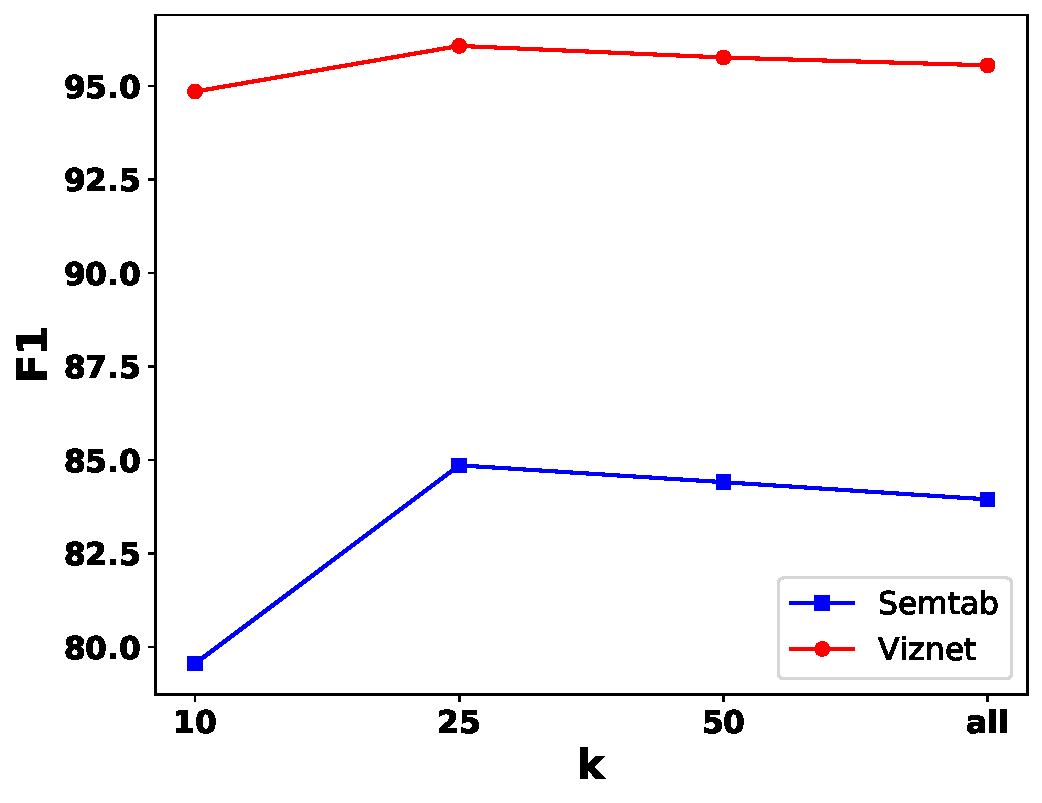
\includegraphics[width=\linewidth]{figures/kglink/F1_k.pdf}
\par\centering\small (a) Weighted F1
\end{minipage}\hfill
\begin{minipage}[b]{0.48\linewidth}
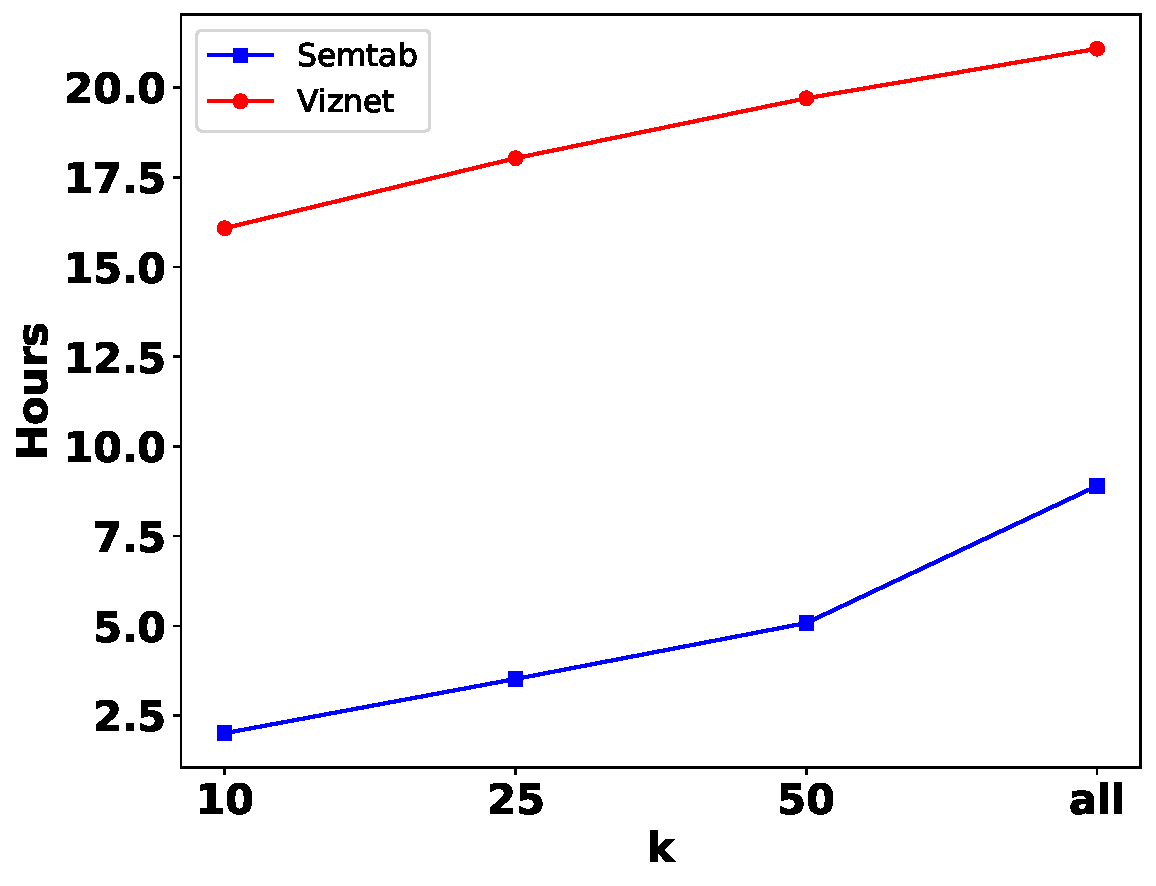
\includegraphics[width=\linewidth]{figures/kglink/k_time.pdf}
\par\centering\small (b) Time cost
\end{minipage}
\caption{Reported effect of the retained row budget $k$. The original two subfigures compare annotation quality and time cost on SemTab and VizNet. Reproduced from KGLink~\cite{kglink-publication}, Fig.~10.}
\label{fig:kglink:row-budget}
\end{figure}

The training-data study uses proportions $p=0.2,0.4,0.6,0.8,1.0$ while keeping the test set unchanged. It compares KGLink with the version without the representation-generation task. The experiment measures data efficiency by varying available supervision against a fixed evaluation set.

\subsection{Runtime in the Evaluated Configuration}
\label{sec:kglink:runtime}

Figure~\ref{fig:kglink:runtime} reproduces the original VizNet runtime chart. KGLink's reported training and inference times are 16.50 and 1.53 hours. The corresponding RECA values are 80.00 and 9.00 hours. The figure also shows methods with shorter measured times, including Doduo at 1.96 hours for training and 0.07 hours for inference. These measurements locate KGLink's annotation results within the costs of the evaluated implementations. Its use of external retrieval and a second training objective carries computation beyond the table encoder alone.

The chart labels MTab's inference entry as N/A. Training and inference times describe different preparation and prediction procedures. The comparison uses VizNet and the original experimental hardware.

The row-budget results address a separate resource decision. They vary how much table content is retained before encoding within KGLink, while the runtime chart compares complete methods. Reading the two studies together identifies the operational choice examined by the chapter. Graph relations determine which evidence enters the encoder, and the retained evidence has a measurable processing cost. The accuracy comparison therefore depends on the selected input and training configuration as well as on the availability of a knowledge graph.

\begin{figure}[tbp]
\centering
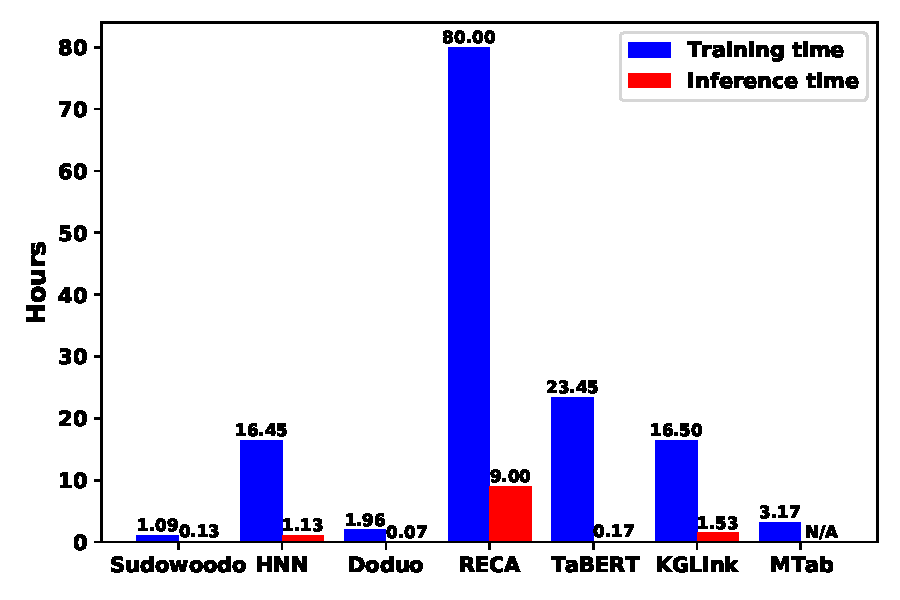
\includegraphics[width=0.9\linewidth]{figures/kglink/runtime.pdf}
\caption{Training and inference time reported on VizNet. Original image reproduced from KGLink~\cite{kglink-publication}, Fig.~7.}
\label{fig:kglink:runtime}
\end{figure}

\section{Discussion and Chapter Summary}
\label{sec:kglink:discussion}

KGLink uses explicit structure at two levels. Within a table row, graph neighborhood connections filter ambiguous entity candidates. Across the rows of a column, recurring graph neighbors support candidate-type selection. These operations determine what external text the encoder receives. The classifier then learns the relation between that evidence and a dataset's label vocabulary. The auxiliary representation task supplies an additional supervised connection between contextual evidence and the intended type description.

The empirical results support this division of responsibilities. The full BERT configuration improves on the version without the masked representation task and on the version without KG information. The row-selection comparison shows that choosing which table values enter the model changes the reported annotation scores. The no-linkage subset confirms that a trained model can continue to annotate tables when the graph stage supplies no retrieved evidence. Each observation corresponds to an explicit component or input condition in the architecture.

Knowledge coverage and annotation vocabulary remain material conditions. The graph-processing stage can use only entities and relations available to its linker and neighborhood retrieval. The supervised predictor learns the type set represented in training. The evaluated datasets use single-label column annotation and bounded table inputs. Those conditions determine the interpretation of the reported accuracy and weighted F1, including why a semantically reasonable graph description can still fail an exact-label evaluation.

The chapter answers the thesis's first research question by showing how graph-derived knowledge can augment a column representation while a learned model handles the target label granularity. The next chapter changes the evidence-maintenance problem. It studies classification when labels and observed examples arrive over successive rounds, using a task-specific graph to retrieve candidate labels and update the available evidence online.
